\documentclass{standalone}
\usepackage{tikz}

\begin{document}

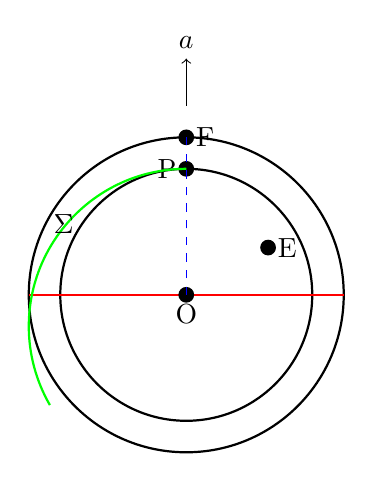
\begin{tikzpicture}[scale=2]
    % Draw the outer circle
    \draw[thick] (0,0) circle (1);
    
    % Draw the inner circle
    \draw[thick] (0,0) circle (0.8);
    
    % Draw the horizontal line
    \draw[red, thick] (-1,0) -- (1,0);
    
    % Mark the center of the circles
    \fill (0,0) circle (0.05) node[below] {O};
    
    % Mark the point F on the outer circle
    \fill (90:1) circle (0.05) node[right] {F};
    
    % Mark the point P on the inner circle
    \fill (90:0.8) circle (0.05) node[left] {P};
    
    % Mark the point E inside the inner circle
    \fill (30:0.6) circle (0.05) node[right] {E};
    
    % Draw the dashed lines from O to F and P
    \draw[dashed, blue] (0,0) -- (90:1);
    \draw[dashed, blue] (0,0) -- (90:0.8);
    
    % Draw the green arc
    \draw[green, thick] (90:0.8) arc (90:90+120:1);
    
    % Label the green arc
    \node at (90+60:0.9) {$\Sigma$};
    
    % Draw the arrow indicating the direction 'a'
    \draw[->, black] (0,1.2) -- (0,1.5) node[above] {$a$};
\end{tikzpicture}

\end{document}